\hypertarget{index_sec_1}{}\section{Aufgabenstellung}\label{index_sec_1}
Die Aufgabenstellung umfasste den Entwurf und den Bau einer Laufmassenwaage mithilfe eines N\-X\-T-\/\-Baukastens, dabei sollte besonderen Wert auf höchstmögliche Präzision gelegt werden. Die Umsetzung sowie der Messbereich der Waage waren den Gruppen freigestellt. \hypertarget{index_sec_2}{}\section{Konzepte}\label{index_sec_2}

\begin{DoxyItemize}
\item Je länger der Hebelarm, desto höher der Messbereich
\item Möglichst leichtes Laufgewicht verwenden um eine hohe Präzision zu gewährleisten
\item Das Laufgewicht langsam fahren lassen um Ausschlag möglichst früh festzustellen und Messungenauigkeiten zu vermeiden
\item Leichtgängigkeit der Wippe um Ausschlag sofort festzustellen 
\end{DoxyItemize}\hypertarget{index_sec_3}{}\section{1. Entwurf}\label{index_sec_3}
Die Idee war es das Laufgewicht möglichst leicht zu halten, indem wir es mit Fäden ziehen. Die Fäden bilden dabei einen Kreislauf, welcher durch ein Rad, das an den Motor angeschlossen ist, angetrieben wird. Das Gewicht wird über die zurückgelegte Distanz des Laufgewichts berechnet. Es wird die Distanz vom Start bis zum Kippen der Wippe benutzt. Die Bewegungen der Wippe werden durch einen Farbsensor bemerkt.

 
\begin{DoxyImage}
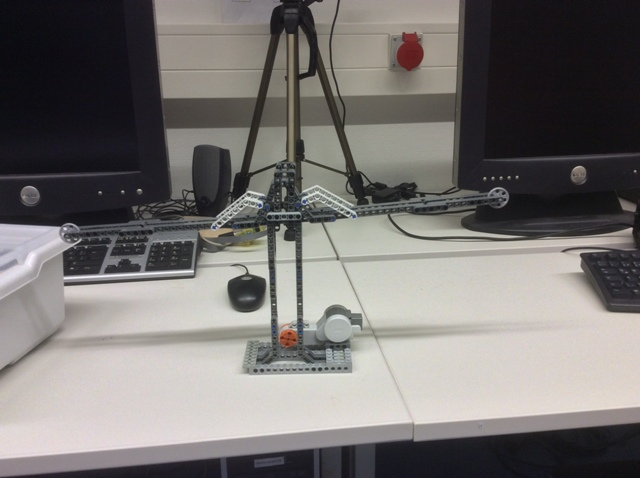
\includegraphics[width=10cm]{entwurf1.jpg}
\caption{Entwurf 1}
\end{DoxyImage}


Probleme\-:
\begin{DoxyItemize}
\item Bei leicht gespannter Schnur rutschte diese bei Belastung über das Antriebsrad
\item Bei stark gespannter Schnur verzog sich das Gestell und genaue Messungen waren unmöglich
\item Ein Kompromiss war schwer umsetzbar
\item Ein anderer Entwurf war nötig 
\end{DoxyItemize}\hypertarget{index_sec_4}{}\section{2. Entwurf}\label{index_sec_4}
Neue Idee, bei der Zahnräder verwendet werden. Das Laufgewicht wird nun nicht mehr durch Schnüre gezogen, sondern wird durch Zahnräder bewegt. Dabei besteht das Laufgewicht aus einem mit Zähnen besetzten Stab, der eine Schiene entlang gleitet. Dadurch sind die vorherigen Probleme behoben.

 
\begin{DoxyImage}
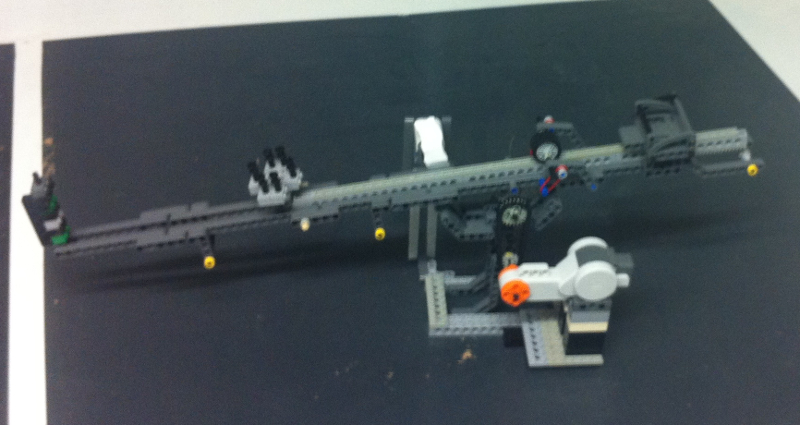
\includegraphics[width=10cm]{entwurf2.jpg}
\caption{Entwurf 2}
\end{DoxyImage}


Probleme\-:
\begin{DoxyItemize}
\item Der Stab könnte durch das Gewicht aus der Schiene springen.
\item Der Ausschlag der Wippe war zu groß
\end{DoxyItemize}

Diese lösten wir durch ein Rad, das leicht von oben auf die Schiene drückt und Halterungen die einen zu großen Ausschlag der Wippe verhindern.

Bisherige Tests verliefen gut, so dass wir uns auf den eigentlichen Messvorgang konzentrierten. Wir testeten mithilfe einer elektronischen Waage und Testgewichte um die ungefähre zurückgelegte Distanz vorhersagen zu können. Dabei werteten wir die Daten aus und generierten eine Funktion, die diese möglichst genau approximiert.\hypertarget{index_sec_5}{}\section{Probleme und Verbesserungen}\label{index_sec_5}
Probleme die immer noch bestehen sind unter anderem\-:
\begin{DoxyItemize}
\item Befestigung des Gewichts spielt eine Rolle für das Messergebnis. Dies würde sich durch ein hängendes Gewicht beheben lassen.
\item Man muss sicherstellen das die Startposition immer dieselbe ist. Das könnte man mithilfe zusätzlicher Sensoren sicherstellen.
\end{DoxyItemize}\hypertarget{index_sec_6}{}\section{Ausblick}\label{index_sec_6}

\begin{DoxyItemize}
\item Veränderung des Messbereiches, durch erhöhen des Laufgewichts.
\item Verlängerung des Hebelarms, um den Messbereich und die Genauigkeit noch weiter zu erhöhen. 
\end{DoxyItemize}